\chapter{Related Work}
\label{c:related}
%%%%%%%%%%%%%%%%%%%%%%%%%%%%%%%%%%%%%%%%%%%%%%%%%%%%%%%%%%%%%%%%%%%%
\section{Backing-Porting}

Two major library in our \RRS{} system:
(1) libbcc: LLVM bitcode compiler and (2) libslang: shim + clang (on-the-host). We show the relation and reference of LLVM compiler library in figure \ref{fig:LLVMRef} and the following sections.

\begin{center-figure}
    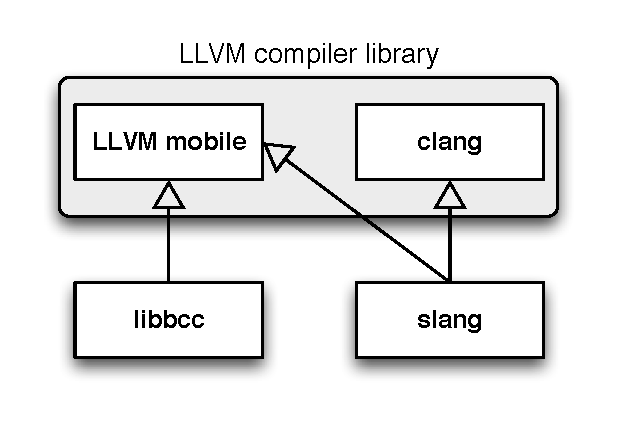
\includegraphics[scale=0.8]{fig/LLVMRef.eps}
    \caption{The referenece of LLVM compiler library}
    \label{fig:LLVMRef}
\end{center-figure}

To deploying \RRS{}, we have to back-port libbcc and libslang from Android Honeycomb to Gingerbread.

Five makefiles are modified for building the whole system:
\begin{enumerate}
    \item \verb|build/core/config.mk|
    \item \verb|build/core/definitions.mk|
    \item \verb|build/core/java.mk|
    \item \verb|build/core/package.mk|
    \item \verb|build/core/prelink-linux-arm.map|
\end{enumerate}

We brief the change as follows:
\paragraph{config.mk} sets up standard variables and other configuration like compiler flags.

\begin{lstlisting}[style=nonumbers]

SLANG := $(HOST_OUT_EXECUTABLES)/llvm-rs-cc$(HOST_EXECUTABLE_SUFFIX)
LLVM_RS_LINK := $(HOST_OUT_EXECUTABLES)/llvm-rs-link$(HOST_EXECUTABLE_SUFFIX)

ifeq ($(HOST_OS),darwin)
HOST_GLOBAL_CFLAGS += -arch i386
HOST_GLOBAL_CPPFLAGS += -arch i386
HOST_GLOBAL_LDFLAGS += -arch i386
endif

\end{lstlisting}

\paragraph{definitions.mk} mostly includes standard commands for building various types of targets, which are used by others to construct the final targes.
\begin{lstlisting}[style=nonumbers]
/**********************************************************
/* Find all of the RenderScript files under the named directories.
/*  Meant to be used like:
/*    SRC_FILES := $(call all-renderscript-files-under,src)
/**********************************************************/

define all-renderscript-files-under
$(patsubst ./%,%, \
   +  $(shell cd $(LOCAL_PATH) ; \
   +          find $(1) -name "*.rs" -and -not -name ".*") \
   +  )
endef

/**********************************************************
/* Commands to compile RenderScript
/***********************************************************/

define transform-renderscripts-to-java-and-bc
@echo "RenderScript: $(PRIVATE_MODULE) <= $(PRIVATE_RS_SOURCE_FILES)"
$(hide) rm -rf $(PRIVATE_RS_OUTPUT_DIR)
$(hide) mkdir -p $(PRIVATE_RS_OUTPUT_DIR)/res/raw
$(hide) mkdir -p $(PRIVATE_RS_OUTPUT_DIR)/src
$(hide) $(SLANG) \
    -o $(PRIVATE_RS_OUTPUT_DIR)/res/raw \
    -p $(PRIVATE_RS_OUTPUT_DIR)/src \
    $(foreach inc,$(PRIVATE_RS_INCLUDES),$(addprefix -I , $(inc))) \
    $(PRIVATE_RS_SOURCE_FILES)
    $(hide) $(LLVM_RS_LINK)    \
    $(PRIVATE_RS_OUTPUT_DIR)/res/raw/*.bc
    $(hide) mkdir -p $(dir $@)
    $(hide) touch $@
\end{lstlisting}

\paragraph{java.mk} takes charge of compiling .java files and .bc files.
\begin{lstlisting}[style=nonumbers]
###############################################################
## .rs files: RenderScript sources to .java files and .bc files
###############################################################
renderscript_sources := $(filter %.rs,$(LOCAL_SRC_FILES))
# Because names of the java files from RenderScript are unknown until the
# .rs file(s) are compiled, we have to depend on a timestamp file.
RenderScript_file_stamp :=
ifneq ($(renderscript_sources),)
renderscript_sources_fullpath := $(addprefix $(LOCAL_PATH)/, $(renderscript_sources))
RenderScript_file_stamp := $(LOCAL_INTERMEDIATE_SOURCE_DIR)/RenderScript.stamp

# prepend the RenderScript system include path
LOCAL_RENDERSCRIPT_INCLUDES := $(TOPDIR)frameworks/base/libs/rs/scriptc \
    $(LOCAL_RENDERSCRIPT_INCLUDES)

$(RenderScript_file_stamp): PRIVATE_RS_INCLUDES := $(LOCAL_RENDERSCRIPT_INCLUDES)
$(RenderScript_file_stamp): PRIVATE_RS_SOURCE_FILES := $(renderscript_sources_fullpath)
# By putting the generated java files into $(LOCAL_INTERMEDIATE_SOURCE_DIR), they will be
# automatically found by the java compiling function transform-java-to-classes.jar.
$(RenderScript_file_stamp): PRIVATE_RS_OUTPUT_DIR := $(LOCAL_INTERMEDIATE_SOURCE_DIR)/renderscript
# TODO: slang support to generate implicit dependency derived from "include" directives.
$(RenderScript_file_stamp): $(renderscript_sources_fullpath) $(SLANG)
   $(transform-renderscripts-to-java-and-bc)

LOCAL_INTERMEDIATE_TARGETS += $(RenderScript_file_stamp)
# Make sure the generated resource will be added to the apk.
LOCAL_RESOURCE_DIR := $(LOCAL_INTERMEDIATE_SOURCE_DIR)/renderscript/res $(LOCAL_RESOURCE_DIR)
endif

# source files generated from RenderScript must be generated before java compiling
ifneq ($(RenderScript_file_stamp),)
$(full_classes_compiled_jar): $(RenderScript_file_stamp)
endif

\end{lstlisting}

\paragraph{package.mk} includes standard rules for building an application package.
\begin{lstlisting}[style=nonumbers]
$(R_file_stamp): $(all_res_assets) $(full_android_manifest) $(RenderScript_file_stamp) $(AAPT) | $(ACP)
$(resource_export_package): $(all_res_assets) $(full_android_manifest) $($(RenderScript_file_stamp)) $(AAPT)
\end{lstlisting}

\paragraph{prelink-linux-arm.map} is a memory-mapping table for prelinking.
\begin{lstlisting}[style=nonumbers]
libbcc.so               0x99000000
\end{lstlisting}
    
%%%%%%%%%%%%%%%%%%%%%%%%%%%%%%%%%%%%%%%%%%%%%%%%%%%%%%%%%%%%%%%%%%%%
\section{slang}

\begin{enumerate}
    \item \textbf{Frontend}: Cleverly reuse Clang abstract syntax tree (AST) to reflect information back to Java layer.
    \item \textbf{Heavey-weight optimizations}: Bcc embeds metadata within bitcode (type, ...) to perform aggressive machine-independent optimizations on host before emitting portable bitcode.
    \item All bitcode supplied as a resource within .apk container.
\end{enumerate}


%%%%%%%%%%%%%%%%%%%%%%%%%%%%%%%%%%%%%%%%%%%%%%%%%%%%%%%%%%%%%%%%%%%%
\section{libbcc}

We shrink the size of LLVM by 10 times smaller to fit in a phone so that we could push frontend + heavy-weight optimizations to slang (in build time).
We do our own Execution engine and JIT, while just leveraging LLVM's low-level codegen libraries and have our 3 debugging mechanisms, so we just removed those big dwarf codes.

For a better Performance:
\begin{itemize}
    \item Fastcc calling convention
    \item VFPv3
    \item Use NEON instead of float4 
    \item Wide range of global, scalar optimizations
    \item 3x speedups over acc 
\end{itemize}
    
Libbcc design:
\begin{itemize}
    \item \textbf{Method-based JIT}: Reasonable scope for optimization.
    \item \textbf{Ahead-of-Time (AOT) compilation}: Caching of EXE cuts launch time.
    \item \textbf{Delta compilation}: Incremental compilation.
    \item \textbf{Modularity:} Each device will have its own JIT. For ARM devices, just include ARM codegen. Same thing for x86, PowerPC, mips devices.
    \item \textbf{On-device linking}: Specialization by CPU/GPU vendors.
    \item \textbf{Reflection}: Inter-operate across languages.
    \item \textbf{Portability}: Many languages target .bc and .bc targets many hardware.
\end{itemize}

%%%%%%%%%%%%%%%%%%%%%%%%%%%%%%%%%%%%%%%%%%%%%%%%%%%%%%%%%%%%%%%%%%%%
\section{LLVM for Android}
For reflection support, we have a tailored version of LLVM(Low Level Virtual Machine) for Android. LLVM\_mobile is ten times smaller than LLVM and three times faster\footnote{more for math-heavy code} than acc\footnote{old \RS{} compiler}.  

LLVM\_mobile is utilized as:
\begin{enumerate}
	\item \textbf{Disassembler} on the phone on the JIT results 	
	\item Android's \textbf{Self-Verifying Native JIT} ─ Three steps to eliminate the human assembler+emulator. First, using Disassembler to debug on assemble code. Second, comparing LLVM assemble code with GCC assemble code for locating where LLVM CodeGen bug is Solution. Third, use Anroid toolchain under prebuilt/ Also users libbcc.so, slang, and modified libElf for compare/verify. It's based on 3 assumptions: (1) Clang/LLVM compile the source and output correct .s; (2) Given a ".s", "as" generates correct binary; (3) ARM instructions can be read as a sequence of unsigned. %http://sourceware.org/bugzilla/show\_bug.cgi?id=11109. Also, other bugs on https://support.codesourcery.com/GNUToolchain/doc6300/getting-started.pdf.
 	\item Standalone \textbf{bcc} mocking RS apis ─ Determine whether a pair of statements is possible to access thread-shared data.
\end{enumerate}

%%%%%%%%%%%%%%%%%%%%%%%%%%%%%%%%%%%%%%%%%%%%%%%%%%%%%%%%%%%%%%%%%%%%
\section{Properties of Android Bitcode}

\begin{enumerate}
	\item ABI-level portability
	\item Basic types, structures and functions
    \item ILP32(Int, Long, and Pointer) , no LP64
    \item Data layout: \\
          \{i32, i32, i32\}: A triple of three i32 values\\
          \{float, i32 (i32) *\}: A pair, the second element is a pointer to a function that takes an i32, returning an i32
    \item Little endian
    \item A portable intermediate representation: \\
          .bc includes target triple in .bc, so runtime JIT can change it.\\
          .bc includes calling convention such as "Arm Architecture Procedure Call Standards"\\
          Bitcode didn't materialize it --> runtime JIT can change it
    \item Alignment: We don't use LLVM default alignments for space/time/GPU concerns. Alignment issues can't resort to runtime JIT, because code may have offsetof()
\end{enumerate}
